\documentclass[tikz,border=8pt]{standalone}
% Shared look for every TikZ diagram. Load with \input{../../tools/tikz-style.tex}
\usepackage[T1]{fontenc}
\usepackage{lmodern}
\renewcommand{\sfdefault}{lmr}  % diagrams use the same serif as the text
\usetikzlibrary{arrows.meta, positioning, shapes.geometric, calc, fit, backgrounds}
\definecolor{cblue}{HTML}{4C78A8}
\definecolor{corange}{HTML}{F58518}
\definecolor{cgreen}{HTML}{54A24B}
\definecolor{cred}{HTML}{E45756}
\definecolor{cpurple}{HTML}{B279A2}
\definecolor{cgrey}{HTML}{6B6B6B}
\tikzset{
  every picture/.style={font=\sffamily, line width=1.2pt},
  box/.style={draw=#1, fill=#1!12, rounded corners=4pt, align=center, inner sep=7pt, minimum height=1.1cm},
  box/.default=cgrey,
  arrow/.style={-{Stealth[length=3mm]}, draw=cgrey, line width=1.4pt},
  title/.style={font=\sffamily\bfseries\Large},
  note/.style={font=\sffamily\small, text=cgrey, align=center},
}
\AtBeginDocument{\hyphenpenalty=10000 \exhyphenpenalty=10000}

% Ray casting in a grid map with 0.5 m cells (drawn coarse for clarity; the Note's code uses 1 mm steps).
% Pose A (2, 2, 0): the forward ray meets the wall cells at x = 5 after 3 m. Pose B (3, 2, 0): after 2 m.
% Reading 1.00 m. Expected ranges: A 3.0 m, B 2.0 m.
\begin{document}
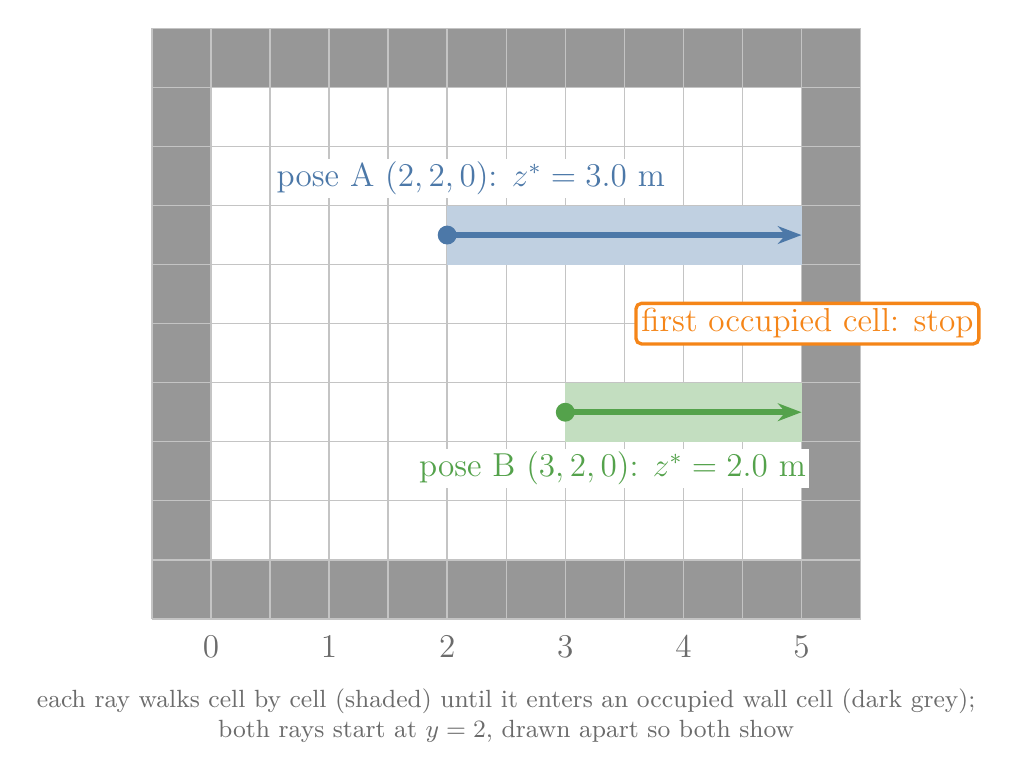
\begin{tikzpicture}[scale=1.5, every node/.append style={font=\large}]
  % occupied wall cells (one ring outside the room)
  \foreach \x in {-0.5,0,...,5} { \fill[cgrey!70] (\x,-0.5) rectangle ++(0.5,0.5); \fill[cgrey!70] (\x,4) rectangle ++(0.5,0.5); }
  \foreach \y in {0,0.5,...,3.5} { \fill[cgrey!70] (-0.5,\y) rectangle ++(0.5,0.5); \fill[cgrey!70] (5,\y) rectangle ++(0.5,0.5); }
  \draw[cgrey!40, line width=0.5pt] (-0.5,-0.5) grid[step=0.5] (5.5,4.5);
  \foreach \x in {0,1,...,5} \node[below, cgrey] at (\x,-0.55) {\x};
  % pose A ray (upper), pose B ray (lower), drawn at y = 2.6 and 1.4 so both show
  \foreach \k in {0,...,5} \fill[cblue!35] (2+\k*0.5,2.5) rectangle ++(0.5,0.5);
  \draw[cblue, line width=2.2pt, -{Stealth[length=3mm]}] (2,2.75) -- (5,2.75);
  \fill[cblue] (2,2.75) circle (0.08);
  \node[cblue, above, fill=white, inner sep=1pt] at (2.2,3.05) {pose A $(2, 2, 0)$: $z^{*} = 3.0$ m};
  \foreach \k in {0,...,3} \fill[cgreen!35] (3+\k*0.5,1.0) rectangle ++(0.5,0.5);
  \draw[cgreen, line width=2.2pt, -{Stealth[length=3mm]}] (3,1.25) -- (5,1.25);
  \fill[cgreen] (3,1.25) circle (0.08);
  \node[cgreen, below, fill=white, inner sep=1pt] at (3.4,0.95) {pose B $(3, 2, 0)$: $z^{*} = 2.0$ m};
  \node[corange, fill=white, inner sep=2pt, draw=corange, rounded corners=2pt] at (5.05,2.0) {first occupied cell: stop};
  \node[note, anchor=north] at (2.5,-1.0) {each ray walks cell by cell (shaded) until it enters an occupied wall cell (dark grey);\\ both rays start at $y = 2$, drawn apart so both show};
\end{tikzpicture}
\end{document}
